\documentclass[11pt,a4paper]{scrartcl}
\usepackage[utf8]{inputenc}
\usepackage[spanish,es-noshorthands]{babel}
\usepackage[margin=2.5cm]{geometry}
\usepackage{graphicx}
\usepackage{amsmath}
\usepackage{booktabs}
\usepackage{float}
\usepackage[hidelinks]{hyperref}

\newcommand{\sig}[1]{\texttt{#1}}

\title{Diseño digital avanzado}
\subtitle{Guía de trabajos prácticos 1}
\author{Krede, Julian}
\date{\today}

\begin{document}
	\maketitle

	\begin{abstract}
		Se describe la resolución de los ejercicios 1 y 4 de la guía. El ejercicio 1 es un
		acumulador de 6 bits con selección de entrada y bandera de overflow; el ejercicio 4
		es un filtro IIR con coeficientes potencia de 2, para el cual se calcula el ancho de
		la salida en \emph{full-resolution} (12 bits). Ambos diseños se verificaron por
		simulación con sus respectivos testbench.
	\end{abstract}

	% ------------------------------------------------------------------
	\section{Ejercicio 1}

	\subsection{Diseño}

	El circuito a implementar (Figura~\ref{fig:ej1_circuito}) es un acumulador: en cada
	flanco ascendente de \sig{clk} se suma al valor guardado en el registro
	(\sig{o\_data}, 6 bits) un valor que depende de \sig{i\_sel}.

	\begin{figure}[H]
		\centering
		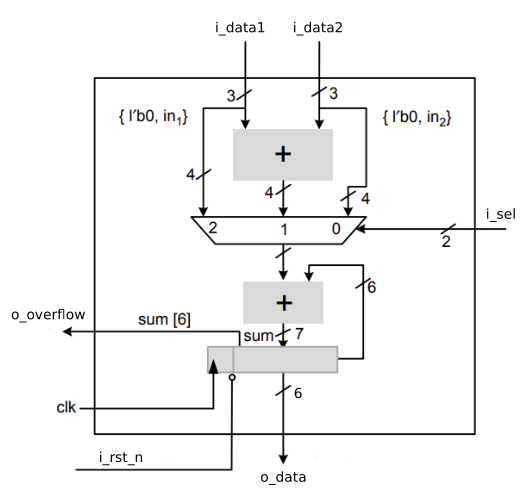
\includegraphics[width=0.6\textwidth]{figuras/ej1_circuito.png}
		\caption{Circuito del ejercicio 1: acumulador con registro de realimentación.}
		\label{fig:ej1_circuito}
	\end{figure}

	Se dividió el camino de datos en un módulo por bloque del diagrama, y \sig{top.v} los
	instancia y conecta:

	\begin{table}[H]
		\centering
		\begin{tabular}{@{}lll@{}}
			\toprule
			Módulo & Bloque del diagrama & Detalle \\
			\midrule
			\sig{adder\_4bits} & Primer sumador & $i\_data1 + i\_data2$, extendidos con ceros a 4 bits \\
			\sig{mux\_3a1}     & Multiplexor    & Elige \sig{\{1'b0,in1\}}, la suma o \sig{\{1'b0,in2\}} \\
			\sig{adder\_7bits} & Segundo sumador & Valor elegido (4 bits) + acumulado (6 bits) \\
			\sig{latch}        & Registro       & Guarda \sig{sum[5:0]} en \sig{o\_data} y \sig{sum[6]} en \sig{o\_overflow} \\
			\bottomrule
		\end{tabular}
	\end{table}

	\begin{table}[H]
		\centering
		\begin{tabular}{@{}cl@{}}
			\toprule
			\sig{i\_sel} & Valor que se suma \\
			\midrule
			\sig{00} & \sig{i\_data1} \\
			\sig{01} & \sig{i\_data1 + i\_data2} \\
			\sig{10} & \sig{i\_data2} \\
			\sig{11} & 0 (la salida se mantiene) \\
			\bottomrule
		\end{tabular}
	\end{table}

	Los anchos siguen el diagrama: la suma de dos números de 3 bits necesita 4 bits para
	no perder el acarreo, y la suma de 4 + 6 bits se hace en 7 bits. Los 6 bits inferiores
	se realimentan al sumador y el bit 6 es el overflow. El código \sig{11} de
	\sig{i\_sel} (no usado en el diagrama) se resolvió con el \sig{default} del
	\sig{case}, que entrega 0 para que el acumulador conserve su valor.

	El registro (\sig{latch.v}, que a pesar del nombre es un flip-flop por flanco) tiene
	\textbf{reset asincrónico activo en bajo}: el \sig{always} es sensible a
	\sig{posedge clk or negedge i\_rst\_n} y con \sig{i\_rst\_n = 0} pone \sig{o\_data} y
	\sig{o\_overflow} en cero sin esperar al reloj.

	\subsection{Testbench}

	El testbench genera un reloj de 10\,ns (100\,MHz), mantiene el reset activo durante
	5 ciclos y lo libera sincronizado con un flanco ascendente, de modo que el registro sale
	del reset en un estado conocido (0) y alineado con el reloj. Después recorre los
	siguientes casos, cada uno durante 10\,µs:

	\begin{enumerate}
		\item \sig{i\_data1 = i\_data2 = 1}, \sig{i\_sel = 01}: medición de ciclos hasta el overflow.
		\item \sig{i\_data2 = 2}, \sig{i\_sel = 10}.
		\item \sig{i\_data1 = 2}, \sig{i\_sel = 00}.
		\item \sig{i\_data1 = 7}, \sig{i\_sel = 00} (máximo de \sig{i\_data1}).
		\item \sig{i\_data2 = 7}, \sig{i\_sel = 10} (máximo de \sig{i\_data2}).
		\item \sig{i\_sel = 11}: la salida debe quedar fija.
	\end{enumerate}

	Los estímulos se cambian después de un \sig{@(posedge clk)} usando asignaciones no
	bloqueantes (\sig{<=}), para que el registro no capture en ese mismo flanco el valor
	nuevo (carrera entre el testbench y el diseño).

	\subsection{Ciclos hasta el overflow}

	Con \sig{i\_sel = 01} y \sig{i\_data1 = i\_data2 = 1} se suma $1+1=2$ en cada flanco.
	Partiendo de 0 (después del reset), luego de $k$ flancos la suma en 7 bits vale $2k$, y
	el bit 6 se pone en 1 cuando la suma llega a $2^6 = 64$:
	\[
		2k \ge 64 \quad\Rightarrow\quad k = 32 \text{ ciclos de reloj.}
	\]

	En la simulación (Figura~\ref{fig:ej1}) el primer flanco que suma es el de 115\,ns y el
	overflow se registra en el de 425\,ns, es decir
	$\frac{425 - 115}{10} + 1 = 32$ flancos, lo que coincide con el cálculo. En ese ciclo
	\sig{o\_data} vuelve a 0 (64 mod 64) y \sig{o\_overflow} queda en 1 durante un solo
	ciclo; a partir de ahí el patrón se repite cada 32 ciclos.

	\begin{figure}[H]
		\centering
		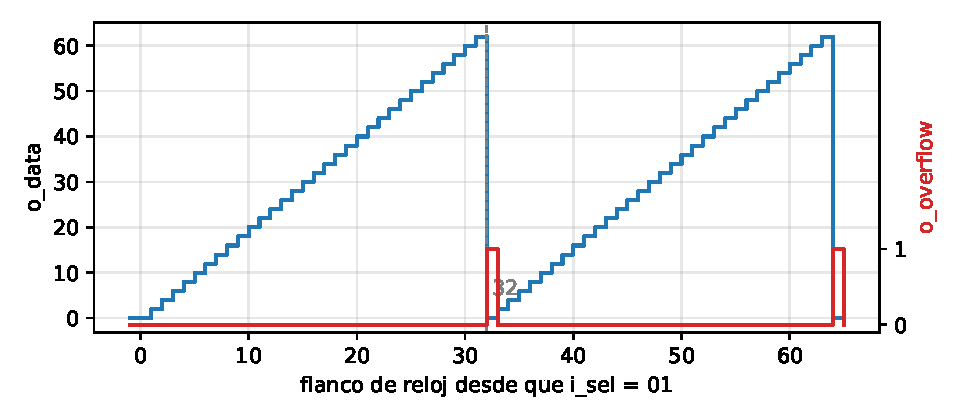
\includegraphics[width=0.85\textwidth]{figuras/ej1_overflow.pdf}
		\caption{Ejercicio 1: \sig{o\_data} y \sig{o\_overflow} con \sig{i\_sel = 01} y ambos datos en 1.}
		\label{fig:ej1}
	\end{figure}

	% ------------------------------------------------------------------
	\section{Ejercicio 4}

	\subsection{Arquitectura}

	El filtro a implementar es
	\[
		y[n] = x[n] - x[n-1] + x[n-2] + x[n-3] + 0{,}5\,y[n-1] + 0{,}25\,y[n-2]
	\]
	con entrada entera de 8 bits en complemento a 2. La arquitectura se dibujó directamente a
	partir de la ecuación (Figura~\ref{fig:filtro}): a la izquierda la parte no recursiva
	(línea de retardo de $x$ y sumadores) y a la derecha la realimentación de $y$.

	\begin{figure}[H]
		\centering
		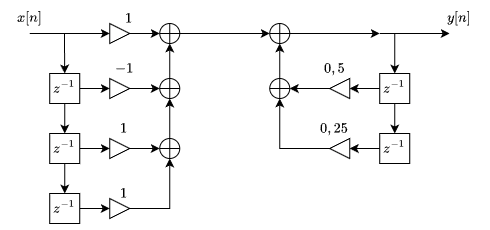
\includegraphics[width=0.8\textwidth]{../Ejercicio4/filtro.png}
		\caption{Arquitectura del filtro.}
		\label{fig:filtro}
	\end{figure}

	Se escribieron tres módulos parametrizables y \sig{top.v} los instancia:

	\begin{itemize}
		\item \sig{registro}: flip-flop con signo, habilitación y reset asincrónico; es
		cada bloque $z^{-1}$. Se usan tres para $x[n-1], x[n-2], x[n-3]$ y dos para
		$y[n-1], y[n-2]$.
		\item \sig{sumador\_restador}: extiende en signo ambos operandos al ancho de salida
		y calcula $a+b$ o $a-b$ según \sig{sub}. El coeficiente $-1$ de $x[n-1]$ se
		implementa como una resta, sin multiplicador.
		\item \sig{mult\_pot2}: multiplica por $2^{-\text{SHIFT}}$ con un desplazamiento
		aritmético (\sig{>>>}), que conserva el signo. Con \sig{SHIFT = 1} se obtiene
		$0{,}5\,y[n-1]$ y con \sig{SHIFT = 2}, $0{,}25\,y[n-2]$.
	\end{itemize}

	El camino de $x[n]$ a $y[n]$ es combinacional; solo las muestras pasadas están
	registradas, así que el filtro no agrega latencia.

	\paragraph{Desplazamiento y truncamiento.} Como las muestras son enteras, el
	desplazamiento a la derecha descarta los bits fraccionarios: \sig{y >>> 1} equivale a
	$\lfloor y/2 \rfloor$ y \sig{y >>> 2} a $\lfloor y/4 \rfloor$. Es un truncamiento hacia
	$-\infty$, con un error de a lo sumo $0{,}5$ y $0{,}75$ respectivamente.

	\subsection{Cálculo de la cantidad de bits de la salida}

	Se pide el ancho de $y$ en \emph{full-resolution}, es decir, el mínimo que garantiza
	que no haya overflow para cualquier secuencia de entrada.

	\paragraph{Datos.} Con $N_x = 8$ bits en complemento a 2, $x[n] \in [-128,\,127]$, y se
	toma como cota de magnitud
	\[
		X_{max} = 2^{N_x-1} = 128 .
	\]
	Los coeficientes de la parte no recursiva son $b = \{1, -1, 1, 1\}$ y los de la
	recursiva $a = \{0{,}5;\ 0{,}25\}$:
	\[
		\sum_k |b_k| = 1+1+1+1 = 4, \qquad \sum_j |a_j| = 0{,}5 + 0{,}25 = 0{,}75 .
	\]

	En la parte no recursiva se podría agregar un bit por sumador, pero la parte recursiva dependen de la propia salida: si se agrega un bit por vuelta al lazo, el ancho crece sin límite. Por eso se plantea una
	cota $M$ tal que $|y[n]| \le M$ para todo $n$ y se pide que sea consistente con la
	ecuación del filtro.

	\paragraph{Cota de la salida.} Aplicando desigualdad triangular a la ecuación y
	reemplazando cada $|x|$ por $X_{max}$ y cada $|y|$ por $M$:
	\begin{align*}
		|y[n]| &\le |x[n]| + |x[n-1]| + |x[n-2]| + |x[n-3]| + 0{,}5\,|y[n-1]| + 0{,}25\,|y[n-2]| \\
		M &\le \underbrace{\Big(\sum_k |b_k|\Big)}_{4} X_{max} + \underbrace{\Big(\sum_j |a_j|\Big)}_{0{,}75} M
		= 4 \cdot 128 + 0{,}75\,M = 512 + 0{,}75\,M .
	\end{align*}
	Despejando $M$:
	\[
		M\,(1 - 0{,}75) = 512 \quad\Rightarrow\quad 0{,}25\,M = 512 \quad\Rightarrow\quad
		M = 2048 .
	\]
	En forma general,
	\[
		M = \frac{\sum_k |b_k|}{1 - \sum_j |a_j|}\, X_{max} = \frac{4}{0{,}25}\cdot 128 = 16 \cdot 128 = 2048,
	\]
	donde el factor $16$ es la ganancia de peor caso del filtro. La cota solo existe si
	$\sum_j |a_j| < 1$ (condición suficiente de estabilidad), que se cumple con
	$0{,}75$.

	\paragraph{Pasaje a bits.} Un número con signo de $N_y$ bits cubre
	$[-2^{N_y-1},\, 2^{N_y-1}-1]$, así que se necesita $2^{N_y-1} \ge M$:
	\[
		N_y = N_x + \left\lceil \log_2\!\left(\frac{\sum_k |b_k|}{1 - \sum_j |a_j|}\right) \right\rceil
		= 8 + \lceil \log_2 16 \rceil = 8 + 4 = \boxed{12 \text{ bits}} .
	\]
	Con 12 bits el rango es $[-2048,\, 2047]$. Como la entrada positiva máxima es 127, la
	salida positiva queda acotada por $16 \cdot 127 = 2032 \le 2047$, y la negativa por
	$-16 \cdot 128 = -2048$, que entra justo en el límite.

	\paragraph{Anchos internos.} En la parte no recursiva cada sumador agrega un bit:
	$x[n]-x[n-1]$ en 9 bits, $+x[n-2]$ en 10 y $+x[n-3]$ en 11 (\sig{NB\_X + 3}). La
	realimentación $0{,}5\,y[n-1] + 0{,}25\,y[n-2]$ y la suma final se hacen en 13 bits
	(\sig{NB\_Y + 1}), y la salida se obtiene tomando los 12 bits inferiores. Descartar el
	bit más significativo es válido porque el cálculo anterior garantiza que el resultado
	siempre entra en 12 bits, de modo que ese bit es solo una copia del signo.

	\subsection{Testbench y resultados}

	El testbench usa el mismo reloj de 10\,ns y deja al menos 1\,µs entre casos para ver la
	respuesta completa. Igual que en el ejercicio 1, \sig{x} se cambia con asignaciones no
	bloqueantes para que el registro de $x[n-1]$ no capture la muestra nueva en el mismo
	flanco. Los casos son: impulso unitario, impulsos de $+127$ y $-128$, escalón de $+127$,
	saltos $+127 \to -128 \to +127$, las secuencias que maximizan y minimizan la parte no
	recursiva, entrada alternada entre los extremos y reset con el filtro cargado.

	La respuesta al impulso de amplitud 127 (Figura~\ref{fig:imp}) coincide con
	$127\,h[n]$, salvo diferencias menores a una unidad debidas al truncamiento:
	$127,\ -64,\ 126,\ 174,\ 118,\ 102,\ \dots$

	\begin{figure}[H]
		\centering
		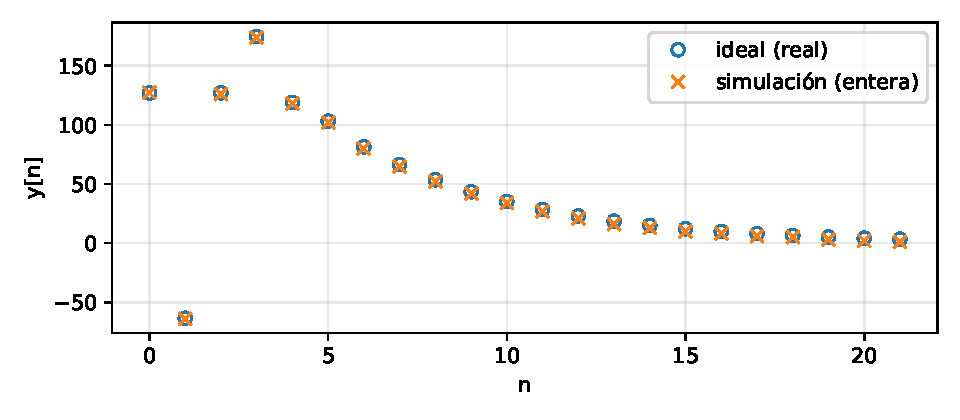
\includegraphics[width=0.85\textwidth]{figuras/ej4_impulso.pdf}
		\caption{Respuesta a un impulso de amplitud 127: valor ideal contra simulación.}
		\label{fig:imp}
	\end{figure}

	Para los escalones (Figura~\ref{fig:esc}) la salida tiende a $H(1)\cdot x = 8x$: con
	$x=-128$ llega exactamente a $-1024$, y con $x = 127$ se estabiliza en $1011$ en lugar
	de $1016$ por el truncamiento de los desplazamientos. En toda la simulación la salida
	quedó en $[-1024,\, 1011]$, dentro del rango de 12 bits, y el reset con el filtro cargado
	lleva la salida a 0.

	\begin{figure}[H]
		\centering
		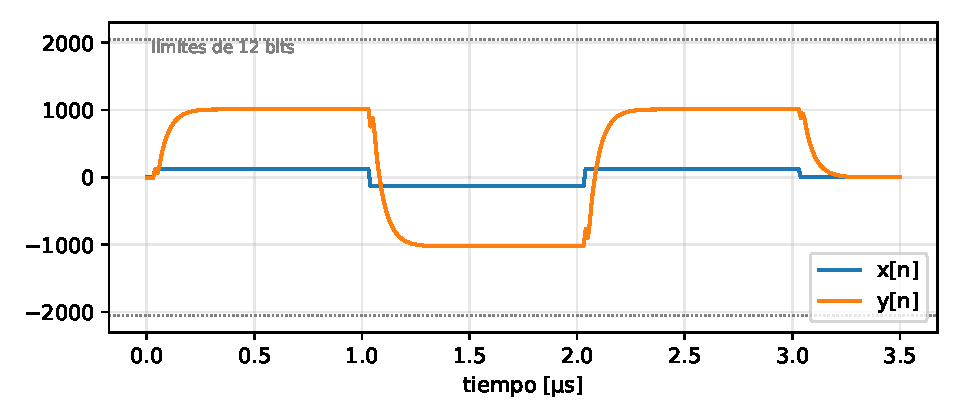
\includegraphics[width=0.85\textwidth]{figuras/ej4_escalon.pdf}
		\caption{Escalones $+127 \to -128 \to +127 \to 0$.}
		\label{fig:esc}
	\end{figure}

	\paragraph{Efecto del truncamiento.} Después del impulso de $-128$ la salida no vuelve a
	0 sino que queda fija en $-5$. Es un ciclo límite que produce el redondeo hacia
	$-\infty$: con $x = 0$,
	\[
		y = \lfloor -5/2 \rfloor + \lfloor -5/4 \rfloor = -3 + (-2) = -5 ,
	\]
	así que $-5$ es un punto fijo. Con valores positivos el truncamiento achica la magnitud y
	la salida sí llega a 0. Si se quisiera eliminar, habría que redondear (sumar medio LSB
	antes de desplazar) o truncar hacia cero.

\end{document}
